\chapter{Cours 1 : Thèmes de théorie des cordes}

\lectureoverview{La bosonisation en dimension \(1+1\), la dualité électrique--magnétique, les D-branes, les transitions à couplage fort, la géométrie émergente et le paysage combinatoire des vides de la théorie des cordes mettent en évidence une difficulté pour le réductionnisme. Un même système physique peut admettre des descriptions élémentaires radicalement différentes ; celle qui paraît simple dépend du couplage et de la géométrie.}

\section{Réductionnisme, complexité et question de la simplicité}

Susskind commence par un slogan philosophique délibérément familier : les grandes choses sont faites de petites choses, et les petites de choses encore plus petites. Il en propose ensuite une version plus ambitieuse, celle qui compte vraiment en physique fondamentale : à mesure que l’on descend vers des couches plus profondes, les objets devraient devenir non seulement plus petits, mais aussi plus simples. Il prend l’image des maisons faites de briques : personne ne confond une maison avec une brique. La brique est plus petite, mais aussi plus simple.

La première étape du cours consiste à confronter cette attente à l’état réel de la physique des particules. Si le réductionnisme apportait une simplicité croissante en ce sens fort, on pourrait s’attendre à ce que la physique des particules élémentaires actuelle soit déjà assez économe. Pourtant, souligne Susskind, même avant d’introduire la gravité quantique, le bilan est déjà compliqué. Dans le cours, ces nombres sont des estimations grossières, mais c’est précisément ce qui sert son propos :
\begin{equation}
\begin{aligned}
N_{\mathrm{species}}&\sim 75,\\
N_{\mathrm{independent}}&\sim 10\text{--}20,\\
N_{\mathrm{parameters}}&\sim 20.
\end{aligned}
\end{equation}
Et ce n’est pas tout. Le Modèle standard ne contient pas la gravité, n’explique pas la matière noire, ne fournit pas la structure supplémentaire nécessaire à l’inflation et présente un grave problème de réglage fin. Ajouter les mécanismes habituels pour y remédier ne fait qu’augmenter le décompte. La supersymétrie en est l’exemple dans le cours. À l’époque, beaucoup de physiciens espéraient que le Grand collisionneur de hadrons mettrait en évidence des superpartenaires ; Susskind souligne que cette extension ajouterait plus d’une centaine de paramètres, au lieu de simplifier immédiatement le bilan. Son message schématique est le suivant :
\begin{equation}
N_{\mathrm{parameters}}^{\mathrm{extended}} \sim 200.
\end{equation}
Ces nombres sont volontairement approximatifs et liés à l’époque du cours. Ils servent à montrer qu’une description plus profonde ne paraît pas nécessairement plus simple lorsqu’on examine l’inventaire des particules et les constantes mesurées.

Cette critique quantitative ne constitue pas encore la thèse principale de Susskind ; elle en est le prélude. L’idée plus profonde, qui guidera la suite du cours, est que la théorie quantique des champs moderne et la théorie des cordes ne semblent pas établir une distinction unique et indépendante du couplage entre les briques et les maisons. Les exemples suivants montrent que ce que l’on entend par ``élémentaire'' peut dépendre des variables les plus efficaces.

\section{La bosonisation : première remise en cause d’une fondamentalité fixe}

Le premier exemple théorique de Susskind vient de la théorie quantique des champs en dimension \(1+1\) : une dimension d’espace et une de temps. Il précise d’emblée qu’il ne va pas démontrer l’équivalence en détail ; l’enjeu n’est pas la preuve formelle, mais la leçon conceptuelle.

On part d’une théorie des champs de fermions. Le champ fermionique est noté \(\psi\). Deux fermions proches peuvent former un composé bosonique, dont le champ correspondant est noté \(\phi\). À première vue, la hiérarchie semble simple : \(\psi\) est fondamental, tandis que \(\phi\) est une variable composite ou effective. Dans le cours, le boson est introduit exactement de cette manière : comme un champ qui crée des paires de fermions liées.

On a toutefois découvert que l’on peut réécrire la même théorie en partant de l’autre extrémité. On peut commencer par le champ bosonique \(\phi\) ; le fermion n’apparaît alors plus comme un constituant ponctuel. Il apparaît plutôt comme un kink du champ bosonique, une configuration étendue dans laquelle \(\phi\) interpole continûment entre deux valeurs asymptotiques. Le contenu mathématique minimal présenté dans le cours est cette structure asymptotique :
\begin{equation}
\phi(x\to -\infty)=\phi_-,
\qquad
\phi(x\to +\infty)=\phi_+.
\end{equation}
Une forme schématique commode est
\begin{equation}
\phi(x)\approx \frac{\phi_++\phi_-}{2}
+
\frac{\phi_+-\phi_-}{2}\tanh\!\left(\frac{x}{\ell}\right),
\end{equation}
où \(\ell\) désigne la largeur de la région de transition.

\editorialnote{Le profil en tangente hyperbolique est une forme lisse standard du kink représenté dans le cours ; la formule n’y est pas dérivée. Le dictionnaire précis de bosonisation dépend du modèle. L’idée conceptuelle est l’échange entre une excitation fermionique et un soliton topologique d’un champ bosonique.}

L’analogie de la ceinture utilisée dans le cours est assez précise pour être conservée. Une ceinture plate, sans torsion, est une configuration sans kink. Si l’on fait tourner une extrémité de \(2\pi\), la ceinture retrouve la même orientation locale loin de la zone de torsion, mais elle doit entre-temps passer par une région torsadée étendue. Cette région est le kink. Dans la description bosonique, le fermion est représenté précisément par un tel objet étendu.

Le propos devient plus net lorsqu’on introduit un couplage. Dans cet exemple, Susskind le note \(G\). Il ne s’agit pas d’un vague lien entre les deux descriptions : leur efficacité dépend du régime du paramètre :
\begin{align}
G \ll 1
&\Rightarrow
\ell\text{ small, tight kink; }\psi\text{ efficient},\\
G \gg 1
&\Rightarrow
\ell\text{ large, broad kink; }\phi\text{ efficient}.
\end{align}
Pour un petit \(G\), le kink est étroit et le fermion paraît être l’objet simple. Quand \(G\) augmente, le kink s’élargit et le fermion devient moins ponctuel. Les variables bosoniques deviennent alors les plus économiques.

\paragraph{Règle d’évolution schématique}
\begin{enumerate}
\item Partir d’une théorie fermionique décrite par \(\psi\).
\item Identifier les composés bosoniques décrits par \(\phi\).
\item Réécrire entièrement la même théorie en fonction de \(\phi\).
\item Dans la description bosonique, le fermion réapparaît sous la forme d’un kink de largeur \(\ell\).
\item Pour \(G\ll 1\), \(\ell\) est petit et la description fermionique est la plus simple.
\item Pour des valeurs plus grandes de \(G\), \(\ell\) augmente et la description bosonique devient la plus simple.
\end{enumerate}

C’est le premier contre-exemple explicite à l’image figée des ``maisons et des briques''. La conclusion du cours n’est pas simplement que des objets composites existent, mais que la variable considérée comme élémentaire peut changer avec le couplage.

\section{Charge électrique, monopôles magnétiques et couplages faible et fort}

Susskind demande ensuite si l’on trouve un phénomène analogue dans une physique des particules plus familière. Son exemple oppose la charge électrique au monopôle magnétique. Dans ce vocabulaire, une particule ordinairement chargée, comme l’électron, est un monopôle électrique : une source localisée de champ électrique. Le monopôle magnétique est introduit par l’analogie avec un aimant droit. Si l’on pouvait isoler l’extrémité d’un tel aimant sans sa barre de liaison invisible, les lignes de champ ressembleraient exactement à celles d’une charge électrique, mais seraient magnétiques plutôt qu’électriques.

Le paramètre de contrôle pertinent est la constante de structure fine \(\alpha\). Dans le cours, Susskind l’interprète de façon heuristique comme le carré de la charge électrique :
\begin{equation}
\alpha \sim e^2.
\end{equation}
Il en donne aussi une interprétation opérationnelle approximative : elle mesure la facilité avec laquelle un électron rayonne. Pour résumer l’intensité de ce rayonnement, il dit qu’un électron accéléré émet de l’ordre de ``\(1/100\)'' photons au sens pertinent ici. Selon les estimations approximatives données dans le cours,
\begin{equation}
\alpha \approx 10^{-2}.
\end{equation}
Il ne s’agit pas d’une convention de précision, mais d’une façon pédagogique de représenter la faiblesse de la charge électrique.

\editorialnote{La relation entre couplages faible--fort a un antécédent précis dans la quantification de Dirac. Dans une convention courante, les charges électrique et magnétique vérifient \(e g_m=2\pi n\). Ainsi, un faible couplage électrique correspond à un fort couplage magnétique, même si les facteurs numériques exacts et les relations de masse protégées dépendent de la théorie.}

Lorsque \(\alpha\ll 1\), l’électron est l’objet simple. Son champ électrique est faible, son nuage de polarisation du vide est dilué et il paraît presque ponctuel. Le monopôle magnétique est alors à l’opposé : son champ est énorme, son environnement est fortement déformé, et il est étendu, complexe et lourd. Susskind résume la situation dans le même esprit, en opposant couplage faible--fort :
\begin{equation}
\begin{aligned}
\alpha \ll 1
&\Rightarrow \text{simple electron;}\\
&\phantom{\Rightarrow{}}\text{heavy, extended monopole},\\
\alpha \gg 1
&\Rightarrow \text{simple monopole;}\\
&\phantom{\Rightarrow{}}\text{heavy, structured electron}.
\end{aligned}
\end{equation}
Le cours ne dérive pas de formule pour la masse du monopôle, car ce n’est pas nécessaire. Le propos est qualitatif. Quand \(\alpha\) augmente, le champ de l’électron se renforce et sa structure s’étoffe, tandis que le monopôle se contracte et s’allège. Bien au-delà de l’unité, les descriptions utiles s’échangent : le monopôle est simple et l’électron, complexe.

C’est la version en théorie des champs de la leçon précédente sur la bosonisation. La distinction entre fondamental et composite n’est pas absolue ; elle dépend du couplage.

\begin{classroomqa}
\audiencequestion{Si le réductionnisme n’est pas un guide fiable, pourquoi les physiciens utilisent-ils le calcul différentiel et intégral, qui semble découper un système en morceaux arbitrairement petits ? \lecturetimestamp{00:21:21}}
\lecturerresponse{Le calcul différentiel et intégral suppose une variation continue ; il ne désigne pas les objets fondamentaux d’une théorie. Les champs quantiques fluctuent à toutes les échelles de distance, ce qui produit une hiérarchie sans fin plutôt qu’une couche lisse ultime où l’on pourrait décider une fois pour toutes ce qui est élémentaire.}
\end{classroomqa}

La discussion se poursuit avec l’idée que cette hiérarchie ressemble à une fractale. Susskind accepte l’analogie, puis la précise : les champs quantiques fluctuent à toutes les échelles et ne sont donc jamais lisses au sens classique. Ces variations excessives contribuent à la difficulté mathématique de la théorie quantique des champs ; il faut utiliser le calcul ordinaire avec des grandeurs renormalisées, plutôt qu’avec un champ microscopique supposé naïvement lisse.

\section{Cordes, D-branes et retour de la dualité faible--fort}

La transition suivante du cours est délibérément naïve. Si la théorie des cordes est censée décrire les briques fondamentales, alors la réponse doit sûrement être simple : les briques sont des cordes. Susskind énonce ouvertement cette attente, puis passe la suite du cours à la déconstruire.

\subsection{Pourquoi les cordes ne suffisent pas}

La première complication tient à la présence inévitable des D-branes. Une D\(p\)-brane est un objet de dimension \(p\) sur lequel les cordes peuvent se terminer. La lettre \(D\) vient des conditions aux limites de Dirichlet, mais ce nom compte bien moins que leur rôle : ces objets font partie de la théorie et on ne peut pas les écarter. Ce ne sont pas des ornements facultatifs.

Les exemples les plus simples sont :
\begin{itemize}
\item une D0-brane, qui est ponctuelle ;
\item une D1-brane, ou corde D, qui a la forme d’une corde ;
\item une corde F, la corde fondamentale ordinaire.
\end{itemize}
Une D0-brane est un site ponctuel lourd où peuvent se terminer un nombre quelconque de cordes F. Une D1-brane est un objet lourd semblable à un câble, beaucoup plus épais et plus massif par unité de longueur qu’une corde F, mais qui peut lui aussi servir de point d’arrivée aux cordes F. À faible couplage, le cours ne présente pas ces objets comme des solutions de rechange tout aussi élémentaires. Les D-branes sont décrites comme des objets lourds, structurés et d’apparence composite, que la théorie nous impose néanmoins.

\editorialnote{La théorie à branes de dimension impaire présentée dans cette partie du cours est la théorie des cordes de type IIB. Ses D-branes stables ont une dimension spatiale impaire, notamment les D1- et D3-branes. Susskind réserve ces noms, car le sujet immédiat est le motif de dualité, et non la classification.}

\paragraph{Notation}
Susskind emploie \(G\) et \(g\) avec une certaine souplesse selon les passages du cours. Ici, \(G\) est réservé à l’exemple de bosonisation, tandis que \(g\) désigne le couplage des cordes.

Le couplage des cordes \(g\) est défini de façon opérationnelle, et non axiomatique. C’est le paramètre qui mesure la probabilité qu’une corde fluctuante se scinde et forme des cordes filles. C’est pourquoi Susskind le compare directement au rôle de \(\alpha\) en électrodynamique quantique. Le cours s’arrête aussi sur la tension, qui correspond à l’énergie par unité de longueur :
\begin{equation}
T=\frac{E}{L}=\frac{M}{L}.
\end{equation}

Pour les cordes F et D, les formules usuelles de la tension rendent explicite la comparaison entre couplages faible--fort :
\begin{equation}
T_{\mathrm{F1}}=\frac{1}{2\pi\alpha'},
\qquad
T_{\mathrm{D1}}=\frac{1}{2\pi\alpha' g_s},
\qquad
\frac{T_{\mathrm{D1}}}{T_{\mathrm{F1}}}=\frac{1}{g_s}.
\end{equation}
\editorialnote{Ces formules de tension donnent la normalisation conventionnelle qui sous-tend la comparaison qualitative du cours entre câble et fil. Elles sont ajoutées par la rédaction ; dans le cours, seul le comportement en fonction du couplage est utilisé.}

\subsection{Cordes F et cordes D}

Le même motif entre couplages faible--fort se répète dans le langage des cordes. À faible couplage, la corde F est légère, mince et proche de l’image intuitive initiale de l’objet fondamental. La corde D est épaisse, lourde et riche en structures de cordes F. Quand le couplage augmente, la corde F se scinde plus facilement ; le nuage de cordes filles prolifère autour d’elle, et elle devient plus lourde et plus complexe. Dans le même temps, la corde D a de plus en plus de mal à émettre les cordes F, désormais lourdes ; sa structure environnante s’amenuise et elle devient plus légère et plus filiforme. Le schéma des couplages faible--fort présenté dans le cours est donc
\begin{align}
g \ll 1
&\Rightarrow
\begin{gathered}
\text{F-string light and thin;}\\
\text{D-string heavy and structured},
\end{gathered}\\
g \sim 1
&\Rightarrow
\text{F-string and D-string comparable},\\
g \gg 1
&\Rightarrow
\begin{gathered}
\text{D-string light and thin;}\\
\text{F-string heavy and structured}.
\end{gathered}
\end{align}
Susskind fait remarquer qu’autour de \(g\sim 1\), les deux descriptions cessent d’être nettement distinctes. Au-delà, elles échangent en pratique leurs rôles. C’est la version de la théorie des cordes de l’échange électron--monopôle, et son nom consacré est la dualité S.

On peut suivre le même échange lorsqu’une corde se referme en boucle. À faible couplage, une petite boucle de corde F est une excitation légère, semblable à une particule, tandis que la boucle de corde D correspondante est lourde et complexe. À fort couplage, leurs rôles s’inversent : la boucle de corde D fournit la description légère, et les excitations légères de corde fermée qui en résultent comprennent le graviton. Susskind s’appuie sur cet exemple pour souligner que l’identité même d’une particule familière peut dépendre du côté de la dualité choisi.

Le cours pousse l’idée un peu plus loin. Dans la théorie idéalisée, le couplage n’est pas simplement un nombre que l’on règle à la main ; il se comporte comme un champ. Schématiquement,
\begin{equation}
g = g(x).
\end{equation}
Différentes régions de l’espace peuvent donc favoriser différentes descriptions duales. Dans une région, les cordes F sont les variables légères ; dans une autre, ce sont les cordes D. Entre les deux, rien n’est particulièrement simple. Pour Susskind, la théorie des cordes ne rétablit donc pas l’image réductionniste simple : elle radicalise l’ambiguïté.

\editorialnote{En théorie des cordes perturbative, le couplage local est déterminé par le dilaton, \(g_s(x)=e^{\Phi(x)}\). Écrire \(g=g(x)\) n’est donc pas une simple analogie, même si les compactifications réalistes produisent généralement un potentiel qui contraint de telles variations.}

\begin{classroomqa}
\audiencequestion{Si le couplage variait suffisamment pour que les cordes D deviennent plus légères que les cordes F dans une autre région, cela modifierait-il les spectres observables ? \lecturetimestamp{00:34:15}}
\lecturerresponse{Oui. C’est l’une des raisons pour lesquelles on ne peut pas identifier directement à notre monde le modèle exactement symétrique et mathématiquement maîtrisé dont il est question. Ses leçons portent sur ce que peuvent faire des théories quantiques cohérentes, et non sur un spectre littéral de la nature.}
\end{classroomqa}

\begin{classroomqa}
\audiencequestion{Existe-t-il une description duale analogue pour une D2-brane ? \lecturetimestamp{00:34:39}}
\lecturerresponse{Oui, mais il ne s’agit pas d’un échange avec une autre corde semblable à la corde D. Le cas des branes de dimension paire mènera à une interprétation en termes de membrane et à une dimension spatiale supplémentaire ; c’est la construction qui suit.}
\end{classroomqa}

\begin{classroomqa}
\audiencequestion{Une probabilité plus élevée de scission des cordes explique-t-elle l’accroissement de la complexité interne ? \lecturetimestamp{00:34:53}}
\lecturerresponse{Oui. Pour rendre le mécanisme concret, revenons à l’électrodynamique quantique : un électron émet des photons, les photons fluctuent en paires chargées, puis les lignes chargées rayonnent à leur tour. Quand le couplage augmente, cette hiérarchie devient moins diluée.}
\end{classroomqa}

\subsection{Retour à l’électrodynamique quantique à partir des questions}

Un étudiant demande alors si la probabilité accrue de scission signifie simplement que la structure est plus complexe «``en amont''». Susskind répond en revenant à l’électrodynamique quantique et en traçant de nouveau la ligne d’univers de l’électron. Ce retour est important : il montre que l’histoire des cordes n’est pas une curiosité isolée, mais une autre manifestation du même motif entre couplages faible--fort.

\begin{figure}[htbp]\centering
\begin{tikzpicture}[scale=1.0]
\draw[->] (-1.2,0) -- (3.7,0) node[right] {space};
\draw[->] (0,-0.2) -- (0,4.3) node[above] {time};

\draw[line width=0.9pt] (0,0.2) -- (0,4.0);
\node[left] at (0,3.55) {\(e^{-}\)};

\draw[line width=0.8pt] (0,1.0) -- (0.18,1.08) -- (0.36,0.92) -- (0.54,1.10) -- (0.72,0.94) -- (0.90,1.12) -- (1.08,0.96) -- (1.26,1.14);
\draw[line width=0.8pt] (0,2.35) -- (-0.18,2.43) -- (-0.36,2.27) -- (-0.54,2.45) -- (-0.72,2.29) -- (-0.90,2.47);

\draw[line width=0.8pt] (1.26,1.14) -- (1.48,1.42);
\draw[line width=0.8pt] (1.26,1.14) -- (1.04,1.42);
\draw[line width=0.8pt] (1.48,1.42) -- (1.58,2.10);
\draw[line width=0.8pt] (1.04,1.42) -- (0.94,2.10);
\draw[line width=0.8pt] (0.94,2.10) -- (1.58,2.10);

\draw[line width=0.7pt] (1.58,1.78) -- (1.72,1.84) -- (1.86,1.72) -- (2.00,1.86);
\draw[line width=0.7pt] (0.94,1.78) -- (0.80,1.84) -- (0.66,1.72) -- (0.52,1.86);

\node at (2.35,1.95) {\(\gamma\)};
\node at (-1.15,2.75) {\(\gamma\)};
\end{tikzpicture}\caption{Hiérarchie schématique en électrodynamique quantique présentée dans le cours : un électron ponctuel émet des photons, les photons créent des paires, puis les lignes chargées filles rayonnent à leur tour, produisant des structures à des échelles toujours plus petites.}\end{figure}

Le cours souligne que même un électron ponctuel s’accompagne d’une hiérarchie de processus :
\begin{enumerate}
\item un électron émet et absorbe des photons ;
\item un photon peut créer une paire électron--positron ;
\item les lignes chargées filles peuvent à leur tour émettre des photons ;
\item la hiérarchie se poursuit vers des échelles plus petites.
\end{enumerate}
À faible couplage, ce nuage est dilué, si bien que l’électron paraît presque ponctuel en laboratoire. À couplage plus fort, il prolifère et l’électron devient un objet structuré. Le cours présente alors l’histoire des cordes comme une analogie directe.

La suite du cours motive aussi le bilan énergétique heuristique de Susskind. Il insiste sur le fait que l’énergie pertinente ne se réduit pas à la somme des contributions des particules libres. Il faut aussi inclure l’énergie d’interaction :
\begin{equation}
E_{\mathrm{tot}} = E_e + E_\gamma + E_{\mathrm{int}}.
\end{equation}
Ici, \(E_{\mathrm{int}}\) est le terme crucial. C’est lui qui permet à la masse de l’électron habillé d’inclure l’énergie associée à son champ environnant et à sa structure virtuelle. Le cours ne transforme pas cette idée en une dérivation formelle de l’auto-énergie renormalisée. Le propos est heuristique, mais essentiel : la masse de l’objet inclut déjà l’énergie d’interaction nécessaire au maintien du nuage complexe qui l’entoure.

\begin{classroomqa}\audiencequestion{D’où vient l’énergie des photons virtuels et des paires électron--positron si un électron ne possède pas assez d’énergie libre pour créer une paire réelle ? \lecturetimestamp{00:37:01}}
\lecturerresponse{On ne part jamais d’un électron nu auquel on ajouterait ensuite son champ coulombien. L’électron observé est un état habillé, et sa masse inclut déjà l’énergie du champ et l’énergie d’interaction. En électrodynamique quantique, l’énergie totale ne se réduit pas à l’énergie de l’électron libre plus celle du photon libre ; le terme d’interaction est indispensable. Il est utile de qualifier les paires intermédiaires de virtuelles, mais le bilan énergétique concerne l’état complet en interaction.}\end{classroomqa}

\begin{classroomqa}\audiencequestion{Lorsqu’une sonde de haute énergie révèle cette structure, l’a-t-elle créée plutôt que mis au jour quelque chose qui était déjà présent ? \lecturetimestamp{00:38:59}}
\lecturerresponse{Cette distinction interprétative peut être débattue. Sur le plan opérationnel, une diffusion à énergie suffisamment élevée donne un état final non trivial que l’on peut calculer. À faible couplage, la plupart des événements paraissent encore simples, tandis qu’une fraction de l’ordre de \(\alpha\) révèle un rayonnement ou des paires supplémentaires.}\end{classroomqa}

\begin{classroomqa}\audiencequestion{Quand on dit que la D1-brane est plus massive que la corde F, sa tension est-elle également plus élevée ? \lecturetimestamp{00:39:37}}
\lecturerresponse{Oui. Pour une corde étendue, « ``masse'' » désigne ici l’énergie par unité de longueur, c’est-à-dire précisément la tension.}\end{classroomqa}

\begin{figure}[htbp]
\centering
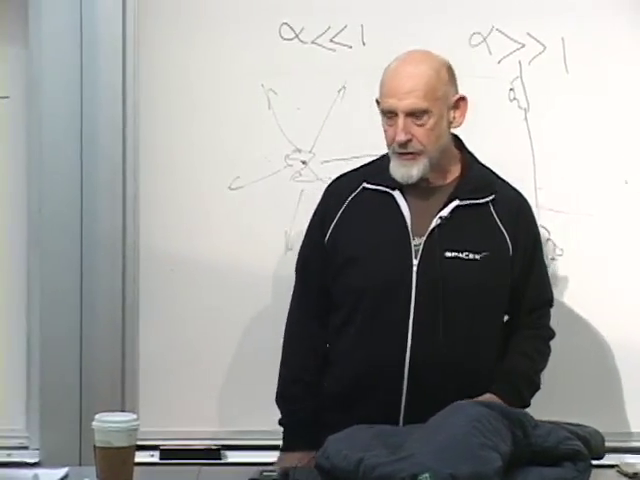
\includegraphics[width=0.72\textwidth]{lecture_01_figure_02.png}
\lectureframe{00:38:22.500}

\vspace{1em}

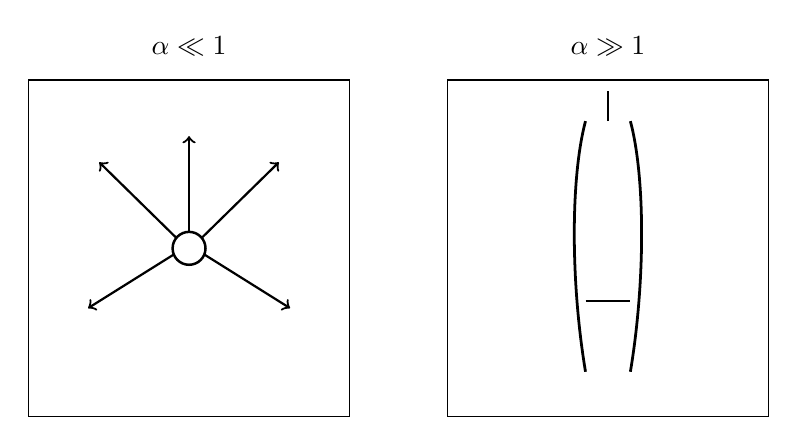
\begin{tikzpicture}[scale=0.95]
\draw (-5.3,-2.4) rectangle (-1.0,2.1);
\draw (0.3,-2.4) rectangle (4.6,2.1);

\node at (-3.15,2.55) {$\alpha \ll 1$};
\node at (2.45,2.55) {$\alpha \gg 1$};

\draw[line width=0.9pt] (-3.15,-0.15) circle (0.22);
\draw[->,line width=0.8pt] (-3.15,0.07) -- (-3.15,1.35);
\draw[->,line width=0.8pt] (-2.98,-0.01) -- (-1.95,1.00);
\draw[->,line width=0.8pt] (-3.32,-0.01) -- (-4.35,1.00);
\draw[->,line width=0.8pt] (-2.95,-0.23) -- (-1.80,-0.95);
\draw[->,line width=0.8pt] (-3.35,-0.23) -- (-4.50,-0.95);

\draw[line width=1.0pt] (2.15,-1.8) .. controls (1.95,-0.6) and (1.95,0.8) .. (2.15,1.55);
\draw[line width=1.0pt] (2.75,-1.8) .. controls (2.95,-0.6) and (2.95,0.8) .. (2.75,1.55);
\draw[line width=0.8pt] (2.15,-0.85) -- (2.75,-0.85);
\draw[line width=0.8pt] (2.45,1.55) -- (2.45,1.95);
\end{tikzpicture}\caption{Comparaison entre couplages faible--fort en électrodynamique quantique pendant la discussion sur l’énergie d’interaction. Le schéma isole les deux régimes évoqués par Susskind : un nuage dilué à faible couplage et un nuage proliférant à fort couplage.}\end{figure}

Cette figure a sa place ici parce que, même si la comparaison entre couplages faible--fort a été introduite plus tôt, Susskind reprend le contraste dans le cours à ce moment ultérieur, à l’occasion d’une question sur l’énergie d’interaction et la prolifération des structures.

\section{Théories à branes de dimension paire et émergence d’une dimension supplémentaire}

Jusqu’ici, le cours a développé l’idée d’échange : fermion contre boson, électron contre monopôle, corde F contre corde D. L’étape suivante est plus surprenante. Susskind passe à une autre version de la théorie des cordes, où les D-branes sont de dimension paire plutôt qu’impaire. Cette distinction compte, car dans cette théorie il n’y a pas de corde D à échanger contre la corde F. On y trouve des D0-branes, des D2-branes, des D4-branes, et ainsi de suite.

La limite de couplage fort ne peut donc pas se réduire à rebaptiser une corde. Selon le cours, il se passe quelque chose de plus étrange : une dimension spatiale supplémentaire devient manifeste. Susskind commence délibérément par la formulation la plus spectaculaire : ---``une nouvelle dimension apparaît''---, puis la reformule aussitôt avec davantage de précision : une direction compacte de très petite taille s’agrandit jusqu’à devenir impossible à négliger.

Le décompte fait partie du propos, aussi Susskind s’y arrête-t-il :
\begin{equation}
\begin{aligned}
10\text{-dimensional string theory} &= 9\text{ space}+1\text{ time},\\
11\text{-dimensional theory} &= 10\text{ space}+1\text{ time}.
\end{aligned}
\end{equation}
Selon le cours, la limite de couplage fort de la théorie à branes de dimension paire est effectivement une théorie à onze dimensions.

\editorialnote{La théorie à branes de dimension paire est la théorie des cordes de type IIA, dont le prolongement à couplage fort est la théorie M. Dans les unités usuelles, le rayon du cercle émergent et la longueur de Planck à onze dimensions varient comme \(R_{11}=g_s\ell_s\) et \(\ell_{11}=g_s^{1/3}\ell_s\). Ces noms et formules explicitent le dictionnaire moderne qui sous-tend la description géométrique du cours.}

\subsection{Le sandwich au beurre de cacahuète}

Pour se représenter la direction compacte, Susskind utilise le modèle du ``sandwich au beurre de cacahuète'' : deux tranches de pain infiniment minces, séparées par un véritable espace. La règle particulière est que sortir d’un côté fait réapparaître de l’autre. Dans une notation conventionnelle, que le cours illustre plutôt qu’il ne formule, on peut écrire
\begin{equation}
y \sim y + 2\pi R.
\end{equation}
Si \(R\) est très petit, les observateurs vivant dans le sandwich décrivent effectivement leur monde comme étant de dimension inférieure. L’effet essentiel du passage au couplage fort est alors
\begin{equation}
g\uparrow
\qquad \Longrightarrow \qquad
R_{\mathrm{compact}}\uparrow.
\end{equation}
Voilà ce que Susskind entend par l’apparition d’une nouvelle dimension spatiale : l’espace n’est pas créé à partir de rien ; une direction compacte jusque-là minuscule s’agrandit et devient visible dans la théorie effective.

\begin{figure}[htbp]\centering
\resizebox{\linewidth}{!}{%
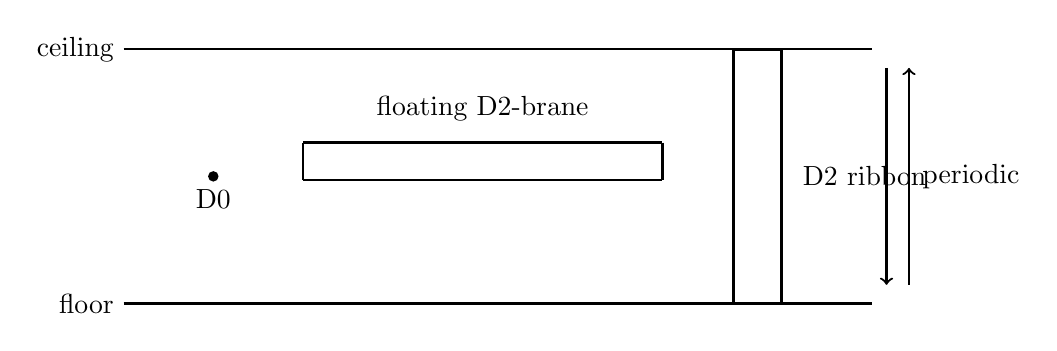
\begin{tikzpicture}[scale=0.95]
\draw[line width=0.9pt] (-5,1.7) -- (5,1.7);
\draw[line width=0.9pt] (-5,-1.7) -- (5,-1.7);

\node[left] at (-5,1.7) {ceiling};
\node[left] at (-5,-1.7) {floor};

\draw[->,line width=0.8pt] (5.2,1.45) -- (5.2,-1.45);
\draw[->,line width=0.8pt] (5.5,-1.45) -- (5.5,1.45);
\node[right] at (5.55,0) {periodic};

\draw[line width=1.0pt] (-2.6,0.45) -- (2.2,0.45);
\draw[line width=1.0pt] (-2.6,-0.05) -- (2.2,-0.05);
\draw[line width=1.0pt] (-2.6,0.45) -- (-2.6,-0.05);
\draw[line width=1.0pt] (2.2,0.45) -- (2.2,-0.05);
\node at (-0.2,0.9) {floating D2-brane};

\draw[line width=1.0pt] (3.15,-1.7) -- (3.8,-1.7);
\draw[line width=1.0pt] (3.15,1.7) -- (3.8,1.7);
\draw[line width=1.0pt] (3.15,-1.7) -- (3.15,1.7);
\draw[line width=1.0pt] (3.8,-1.7) -- (3.8,1.7);
\node[right] at (3.95,0) {D2 ribbon};

\fill (-3.8,0) circle (0.07);
\node[below] at (-3.8,-0.05) {D0};
\end{tikzpicture}}%
\caption{Compactification en sandwich. Les bords supérieur et inférieur sont identifiés périodiquement ; une D2-brane flotte entre eux comme un tapis, tandis qu’une autre s’étend du sol au plafond et ressemble à une corde lorsque la direction compacte est de petite taille.}\end{figure}

\subsection{Que deviennent les D0- et D2-branes ?}

Le cours demande maintenant ce qui advient des D0-branes et des cordes. La réponse est asymétrique. Quand \(g\) devient grand, les D0-branes s’allègent de plus en plus ; dans l’interprétation en dimension supérieure, elles rejoignent la tour des particules porteuses de quantité de mouvement dans la direction nouvellement manifeste. Ainsi, un objet lourd et complexe dans la description à faible couplage devient une excitation ordinaire et légère dans celle à fort couplage.

La relation de masse explicite cette identification :
\begin{equation}
M_{D0}(n)=\frac{n}{g_s\ell_s}
=\frac{n}{R_{11}}
=M_{\mathrm{KK}}(n).
\end{equation}
\editorialnote{Susskind appelle les D0-branes « ``les gravitons'' » de la théorie à onze dimensions. Plus précisément, leurs états liés sont les modes de quantité de mouvement de Kaluza--Klein du multiplet de supergravité à onze dimensions, dont le secteur sans masse contient le graviton. Cette distinction conserve l’identification physique du cours sans aller jusqu’à affirmer littéralement qu’il s’agit d’une seule particule.}

Les D2-branes expliquent ce qu’il advient des cordes. Le cours met en avant deux configurations :
\begin{enumerate}
\item une D2-brane flottant entre le sol et le plafond comme un tapis dans le beurre de cacahuète ;
\item une D2-brane tendue du sol au plafond comme un ruban, étendu dans la direction visible.
\end{enumerate}
Lorsque le sandwich est mince, le ruban paraît effectivement unidimensionnel. C’est l’objet que les observateurs à basse énergie appellent une corde. À mesure que la direction compacte s’ouvre, ce même objet prend nettement la forme d’une membrane. Comme il s’étend désormais davantage dans la direction verticale, il devient lourd et ne ressemble plus à une corde.

\paragraph{La logique de la transition.}
\begin{enumerate}
\item Partons d’une direction compacte très mince, de sorte que le ruban vertical se comporte effectivement comme une corde.
\item Augmentons \(g\) : la direction compacte s’agrandit.
\item Les D0-branes s’allègent et sont réinterprétées comme des états de quantité de mouvement de Kaluza--Klein dans la théorie de dimension supérieure.
\item Le ruban de D2, semblable à une corde, devient une membrane visiblement étendue et s’alourdit.
\end{enumerate}
C’est le point d’articulation du cours entre dualité et géométrie émergente. Le couplage fort ne se contente pas d’échanger un objet contre un autre : il change la géométrie qui offre la description la plus efficace.

Susskind s’arrête sur l’étrangeté de cette idée. Le réseau d’identifications proposées exigeait de difficiles relations de cohérence mathématique, dont certaines ont d’abord été avancées par les physiciens sous forme de conjectures, puis démontrées par les mathématiciens. Il ne prétend pas que l’on comprend tous les vide de corde réalistes, mais que le réseau de dualités lui-même a résisté à des vérifications d’une rigueur inhabituelle.

Si le couplage varie d’un endroit à l’autre dans ce cadre idéalisé, la géométrie la plus efficace peut varier avec lui. Une région peut sembler presque de dimension dix, avec des cordes légères et des D0-branes lourdes ; une autre peut s’ouvrir sur la description de dimension onze, avec des membranes enroulées lourdes et des modes de Kaluza--Klein légers. Ce changement local de langage fait partie du même réseau de dualités.

La transcription rend brièvement le nom de ces relations par ``inégalités.'' Dans ce contexte, le mot visé est \emph{dualités} : des relations entre les deux extrémités opposées de l’espace des paramètres. Cette correction importe, car la conclusion de la leçon est précisément que l’on ne connaît aucune liste unique de constituants fondamentaux. Cordes, branes, particules et géométrie de dimension supérieure peuvent se transformer les uns dans les autres ; soit aucun élément du réseau n’est absolument fondamental, soit il existe une organisation plus profonde qui demeure inconnue.

\section{D3-branes, membranes enroulées et représentation géométrique de la dualité}

Après la pause, Susskind décrit explicitement le sujet comme un ``vaste réseau'' de théories et d’idées interconnectées. Les exemples qui suivent ne sont pas de nouveaux effets isolés ; ce sont des ponts qui relient les exemples précédents.

\subsection{Le volume d’univers d’une D3-brane}

Le premier pont fait intervenir une D3-brane. Une D3-brane possède trois dimensions spatiales et un observateur qui y est confiné peut facilement la prendre pour l’espace ordinaire. La brane peut se courber et fluctuer, tandis que les cordes qui s’y terminent peuvent se joindre, se scinder et diffuser. Pour un observateur qui ne voit que les directions le long de la brane, chaque extrémité ressemble à une particule et les interactions entre ces extrémités à celles d’une théorie quantique des champs ordinaire.

\begin{figure}[htbp]
\centering
\resizebox{\linewidth}{!}{%
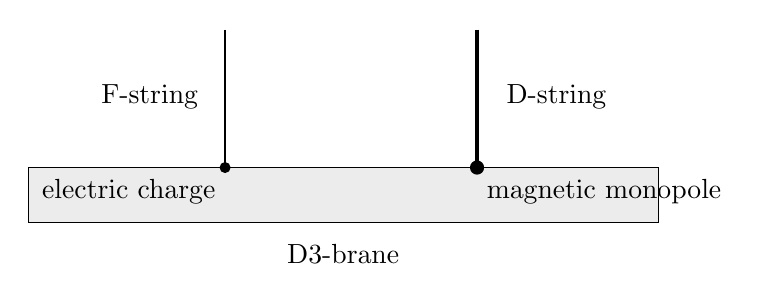
\begin{tikzpicture}[scale=1.0]
\draw[fill=gray!15] (-4,-0.35) rectangle (4,0.35);
\node at (0,-0.75) {D3-brane};

\draw[line width=0.9pt] (-1.5,2.1) -- (-1.5,0.35);
\fill (-1.5,0.35) circle (0.07);
\node[left] at (-1.72,1.25) {F-string};
\node[below left] at (-1.5,0.32) {electric charge};

\draw[line width=1.5pt] (1.7,2.1) -- (1.7,0.35);
\fill (1.7,0.35) circle (0.09);
\node[right] at (1.95,1.25) {D-string};
\node[below right] at (1.7,0.32) {magnetic monopole};
\end{tikzpicture}
}%
\caption{Interprétation en termes de volume d’univers d’une D3-brane. L’extrémité d’une corde F apparaît comme une charge électrique ; celle d’une corde D apparaît comme un monopôle magnétique.}
\end{figure}

C’est l’une des identifications les plus satisfaisantes de la leçon. Pour l’observateur du volume d’univers, une corde F qui se termine sur la D3-brane apparaît comme une charge électrique. Une corde D se terminant sur cette même brane apparaît comme un monopôle magnétique. Autrement dit, sur le volume d’univers de la D3-brane, la dualité entre cordes F et cordes D devient la dualité électrique--magnétique de la théorie des champs ordinaire. Ce qui n’était auparavant qu’une analogie devient un dictionnaire explicite.

\editorialnote{Pour un empilement de D3-branes, la description à basse énergie sur le volume d’univers est une théorie de Yang--Mills supersymétrique en quatre dimensions, avec \(\mathcal N=4\). Sa dualité électrique--magnétique réalise, dans la théorie des champs, la dualité S de type IIB ; une brane unique donne la limite abélienne illustrée dans le cours.}

\subsection{Deux directions compactes et un enroulement asymétrique}

Susskind revient ensuite à la géométrie de dimension supérieure et compacte non pas une, mais deux petites directions. Comme on ne peut pas dessiner onze dimensions au tableau, il représente par une seule direction horizontale visible les sept grandes directions qui ne figurent pas dans le schéma, puis dessine explicitement les deux directions compactes. Il insiste sur l’asymétrie de la compactification : l’une des directions compactes doit être plus courte que l’autre pour que les cordes effectives aient des tensions différentes.

\begin{figure}[htbp]
\centering
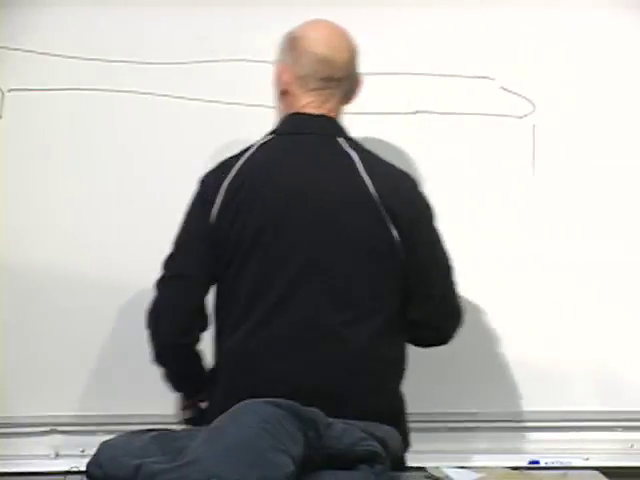
\includegraphics[width=0.78\textwidth]{lecture_01_figure_03.png}
\lectureframe{01:10:25.000}
\caption{État final du schéma au tableau pour les deux membranes enroulées. Les cycles compact court et long produisent les rubans de type corde F et corde D dessinés à droite.}
\end{figure}

Une membrane peut s’enrouler autour de l’une ou l’autre des directions compactes et apparaître comme une corde dans les directions non compactes. Si \(R_1\) et \(R_2\) sont les rayons des deux cercles, ses tensions effectives sont
\begin{equation}
\begin{aligned}
T_{(1)}&=2\pi R_1 T_{\mathrm{M2}},\\
T_{(2)}&=2\pi R_2 T_{\mathrm{M2}},\\
\frac{T_{(1)}}{T_{(2)}}&=\frac{R_1}{R_2}.
\end{aligned}
\end{equation}
Ainsi, des cercles de tailles différentes produisent des tensions de corde différentes. En identifiant l’enroulement le plus court à la corde F légère et le plus long à la corde D lourde, on peut écrire schématiquement
\begin{equation}
g_s\sim \frac{R_{\mathrm{short}}}{R_{\mathrm{long}}},
\qquad
\frac{T_{\mathrm{D1}}}{T_{\mathrm{F1}}}\sim \frac{1}{g_s}.
\end{equation}

\begin{classroomqa}
\audiencequestion{Dans ce schéma, le couplage peut-il s’interpréter comme le rapport des deux dimensions compactes ? \lecturetimestamp{01:10:13}}
\lecturerresponse{Oui. Le paramètre faible--fort est géométrisé sous la forme d’un rapport d’aspect. Rendre une direction plus courte donne un faible couplage ; échanger les deux directions revient à échanger les cordes légère et lourde.}
\end{classroomqa}

\editorialnote{Dans la leçon, ce rapport est provisoirement noté \(\alpha\), le symbole précédemment utilisé pour la constante de structure fine de l’électrodynamique quantique. Nous écrivons ici \(g_s\) pour distinguer les deux significations. Dans la construction complète de la théorie M, le couplage de type IIB est encodé dans la structure complexe du tore compact à deux dimensions ; le numérateur précis dépend de la manière dont ses cycles sont étiquetés.}

On peut résumer la représentation par membranes enroulées sans la distorsion de perspective du dessin au tableau :

\begin{figure}[htbp]
\centering
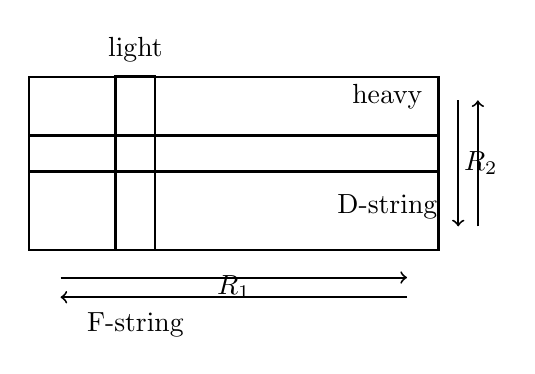
\begin{tikzpicture}[scale=1.0]
\draw[line width=0.9pt] (0,0) rectangle (5.2,2.2);
\node[below] at (2.6,-0.2) {\(R_1\)};
\node[right] at (5.4,1.1) {\(R_2\)};

\draw[->,line width=0.7pt] (5.45,1.9) -- (5.45,0.3);
\draw[->,line width=0.7pt] (5.7,0.3) -- (5.7,1.9);
\draw[->,line width=0.7pt] (0.4,-0.35) -- (4.8,-0.35);
\draw[->,line width=0.7pt] (4.8,-0.6) -- (0.4,-0.6);

\draw[line width=1.0pt] (1.1,0) -- (1.6,0) -- (1.6,2.2) -- (1.1,2.2) -- cycle;
\node at (1.35,2.55) {light};

\draw[line width=1.0pt] (0,1.45) -- (5.2,1.45);
\draw[line width=1.0pt] (0,1.00) -- (5.2,1.00);
\node at (4.55,1.95) {heavy};

\node at (1.35,-0.95) {F-string};
\node at (4.55,0.55) {D-string};
\end{tikzpicture}
\caption{Deux configurations de membranes enroulées semblent toutes deux être des cordes dans les directions non compactes, mais la différence d’échelle des directions compactes rend l’une des cordes effectives plus légère que l’autre.}
\end{figure}

C’est la version géométrique du récit de dualité précédent. Comprimer une direction tout en étirant l’autre alourdit un objet enroulé et allège l’autre, de sorte que les rôles des cordes F et D peuvent s’inverser.

\begin{classroomqa}
\audiencequestion{Si les directions compactes sont cycliques, les objets enroulés sont-ils infiniment larges ? \lecturetimestamp{01:10:41}}
\lecturerresponse{Non. Un cercle compact a une circonférence finie, même si l’on peut le parcourir indéfiniment sans rencontrer de bord. Le haut et le bas du dessin déroulé représentent le même point, tout comme les extrémités d’un intervalle peuvent représenter un seul point d’un cercle.}
\end{classroomqa}

\begin{figure}[htbp]
\centering
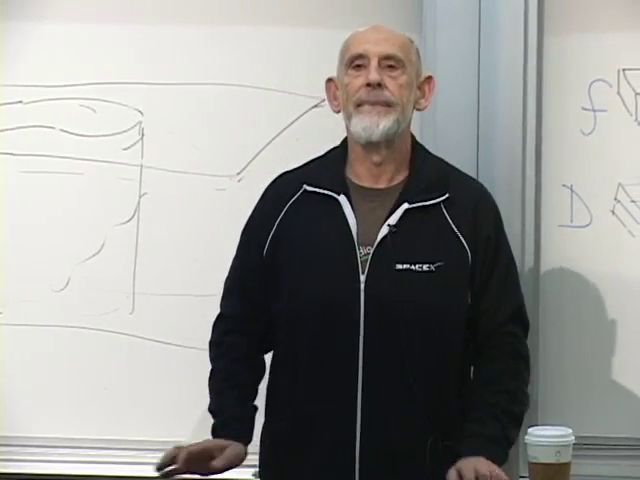
\includegraphics[width=0.78\textwidth]{lecture_01_figure_04.png}
\lectureframe{01:12:25.000}

\vspace{1em}

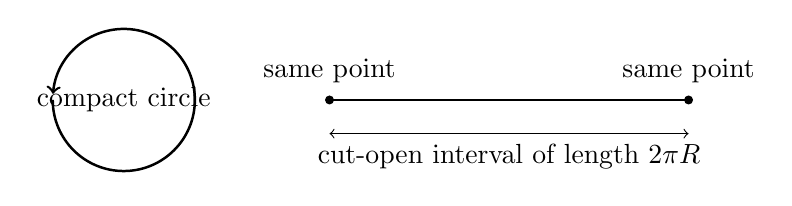
\begin{tikzpicture}[scale=0.95]
\draw[line width=0.9pt,->] (-3.7,0) arc[start angle=180,end angle=535,radius=0.95];
\node at (-2.75,0) {compact circle};
\draw[line width=0.9pt] (0.0,0) -- (4.8,0);
\fill (0.0,0) circle (0.06);
\fill (4.8,0) circle (0.06);
\draw[<->] (0.0,-0.45) -- (4.8,-0.45);
\node at (2.4,-0.75) {cut-open interval of length \(2\pi R\)};
\node[above] at (0.0,0.1) {same point};
\node[above] at (4.8,0.1) {same point};
\end{tikzpicture}
\caption{Un cercle compact et sa représentation déroulée au tableau. En franchissant une extrémité, on revient par l’autre ; se déplacer autour du cercle tout en avançant dans une direction non compacte tracerait plutôt une hélice.}
\end{figure}

\begin{classroomqa}
\audiencequestion{Pourquoi le chemin compact est-il un cercle plutôt qu’une hélice ? \lecturetimestamp{01:12:23}}
\lecturerresponse{En chaque point fixe de la direction non compacte, la direction compacte est un cercle. Une hélice n’apparaît que si l’on avance dans la direction non compacte tout en s’enroulant autour du cercle. L’intervalle dessiné au tableau est simplement un cercle coupé, dont les deux extrémités sont identifiées.}
\end{classroomqa}

\begin{classroomqa}
\audiencequestion{Cette géométrie explique-t-elle à elle seule comment une D-brane peut ressembler à un ensemble de cordes F lorsqu’on la sonde de près ? \lecturetimestamp{01:12:49}}
\lecturerresponse{Le lien existe, mais il n’est pas manifeste dans cette représentation élémentaire ; il faut un outillage géométrique plus élaboré pour le voir. Le schéma sert à organiser la dualité, pas à dériver la description de tous les constituants microscopiques.}
\end{classroomqa}

\begin{classroomqa}
\audiencequestion{Les directions compactes longue et courte peuvent-elles s’échanger lorsqu’on se déplace dans l’espace ou au cours du temps ? \lecturetimestamp{01:13:35}}
\lecturerresponse{L’un ou l’autre est possible dans le modèle idéalisé. Comprimer un cycle tout en dilatant l’autre inverse lequel des cordes enroulées est léger. C’est une autre raison pour laquelle ``corde fondamentale'' n’est qu’un nom : la description privilégiée peut changer d’une région à l’autre ou au cours du temps.}
\end{classroomqa}

\section{Idéalisation, points de symétrie particulière et paysage}

Dans le dernier mouvement de la leçon, Susskind prend du recul par rapport aux élégants exemples de dualité et se demande ce qu’ils nous apprennent — et ce qu’ils ne nous apprennent pas — sur le monde réel.

Tout d’abord, Susskind avertit que les dualités précisément contrôlées sont des propriétés de théories supersymétriques fortement idéalisées, dans lesquelles bosons et fermions ont des masses exactement égales. Il les compare aux orbites circulaires de la mécanique newtonienne : on les étudie d’abord parce qu’elles sont symétriques et mathématiquement faciles à traiter, non parce que le mouvement réel des planètes se réduit à des cercles parfaits. De même, les théories des cordes supersymétriques sont plus faciles à analyser parce qu’elles sont plus symétriques que ne semble l’être la nature.

Cette idéalisation n’en est pas moins instructive. Une orbite circulaire parfaite ne représente pas un système planétaire réaliste, mais elle met en évidence des propriétés qui subsistent pour des orbites moins symétriques. De même, les exemples supersymétriques montrent des façons cohérentes d’articuler la mécanique quantique, la gravité et la structure microscopique. Susskind formule délibérément les choses de manière tranchée : littéralement, les théories des cordes traitables ne sont pas la théorie de notre monde ; elles sont utiles parce qu’elles révèlent des phénomènes susceptibles de réapparaître dans des cadres moins symétriques et moins faciles à traiter.

\subsection{Un ensemble de briques de construction aux nombreuses issues}

Les D-branes ne sont qu’un élément de l’ensemble de briques de construction disponible. La leçon mentionne aussi les flux, les orbifolds et les orientifolds. On choisit d’abord une géométrie compacte, puis les branes et les flux qui occupent ses cycles. Même le simple sandwich change de physique à basse dimension lorsqu’on y insère une, deux ou trois D2-branes flottantes. Ajouter ou retirer de tels ingrédients modifie les particules, les interactions et les paramètres effectifs.

Supposons que, dans le décompte schématique de la leçon, un espace compact à six dimensions possède environ \(500\) cycles, et que chaque cycle admette de l’ordre de \(10\) possibilités de branes enroulées, de flux ou de structures apparentées. Le nombre de constructions croît alors comme
\begin{equation}
N_{\mathrm{vacua}} \sim 10^{500}.
\end{equation}
Le raisonnement de la leçon est élémentaire :
\begin{equation}
10 \times 10 \times \cdots \times 10 = 10^{500}
\end{equation}
avec \(500\) facteurs. L’analogie avec l’ADN exprime la même idée dans un registre plus familier :
\begin{equation}
N_{\mathrm{DNA}}(500)=4^{500}.
\end{equation}
Lors de la comparaison avec l’ADN, un membre du public vérifie qu’il y a quatre possibilités le long d’un brin : A, C, G et T. Cette correction renforce l’argument sans le modifier. Une courte liste de choix locaux, répétée de nombreuses fois, produit un nombre immense d’arrangements globaux. L’exposant exact n’est pas le point essentiel, et Susskind qualifie \(10^{500}\) de vieille sous-estimation ; l’essentiel est la prolifération combinatoire.

On aboutit ainsi à l’inversion finale de l’attente réductionniste formulée au début. Une physique des particules complexe ne nécessite pas forcément des règles microscopiques complexes. Elle peut résulter du fait que notre vide est un arrangement complexe de nombreux ingrédients simples, tout comme un organisme complexe peut être encodé par une séquence constituée de quatre bases.

\begin{classroomqa}
\audiencequestion{Une fois identifiées les descriptions équivalentes liées par dualité, une connaissance complète permettrait-elle de ne retenir qu’un seul de ces vides possibles, ou quelques-uns, comme descriptions de notre monde ? \lecturetimestamp{01:26:11}}
\lecturerresponse{On peut présumer qu’elle sélectionnerait un ensemble restreint, mais de nombreux vides distincts pourraient sembler extrêmement semblables aux énergies accessibles. Le nombre cité pour le paysage est censé rester élevé même après identification des descriptions duales, et les détails de haute énergie sans pertinence pourraient jouer le rôle de ``l’ADN poubelle.''}
\end{classroomqa}

\subsection{Points de symétrie et complexité générique}

Dans le paysage, il existe des points présentant une symétrie particulière. Dans la représentation géométrique, une configuration de rapport d’aspect égal,
\begin{equation}
R_1=R_2,
\end{equation}
rend les deux descriptions par enroulement aussi simples l’une que l’autre. Dans l’analogie électrique--magnétique, cela se représente schématiquement par
\begin{equation}
m_{\mathrm{monopole}}=m_e.
\end{equation}

\begin{figure}[htbp]
\centering
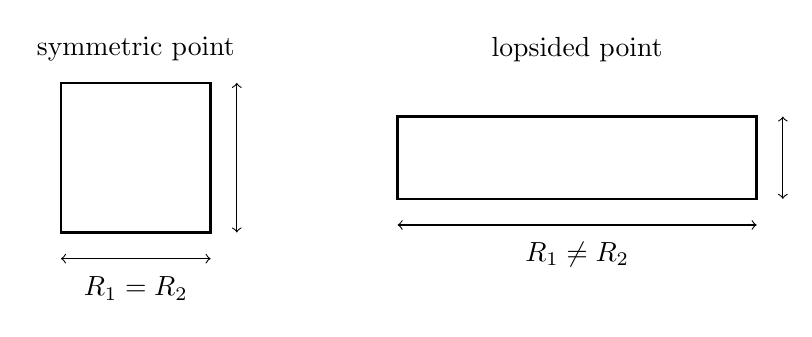
\begin{tikzpicture}[scale=0.95]
\draw[line width=0.9pt] (-4.5,-1.0) rectangle (-2.5,1.0);
\draw[<->] (-4.5,-1.35) -- (-2.5,-1.35);
\draw[<->] (-2.15,-1.0) -- (-2.15,1.0);
\node at (-3.5,1.45) {symmetric point};
\node at (-3.5,-1.75) {$R_1=R_2$};

\draw[line width=0.9pt] (0.0,-0.55) rectangle (4.8,0.55);
\draw[<->] (0.0,-0.9) -- (4.8,-0.9);
\draw[<->] (5.15,-0.55) -- (5.15,0.55);
\node at (2.4,1.45) {lopsided point};
\node at (2.4,-1.3) {$R_1\ne R_2$};
\end{tikzpicture}
\caption{Une compactification de rapport d’aspect égal traite symétriquement les deux cordes enroulées ; une compactification dissymétrique rend l’une des descriptions beaucoup plus légère que l’autre.}
\end{figure}

\begin{classroomqa}
\audiencequestion{Existe-t-il dans le paysage des vides où la construction devient beaucoup plus simple parce que les descriptions en termes de cordes F et D coïncident ? \lecturetimestamp{01:27:21}}
\lecturerresponse{Oui, il existe des points présentant une symétrie particulière. Notre monde ne semble pas se trouver en l’un d’eux : la particule électrique familière et le monopôle magnétique n’ont pas la même masse. On ignore pourquoi la nature occupe un point dissymétrique.}
\end{classroomqa}

\editorialnote{L’égalité des masses de l’électron et du monopôle-- est une propriété schématique d’un modèle autodual convenablement protégé, et non une prédiction de l’électrodynamique quantique ordinaire non supersymétrique. Elle exprime l’idée du point de symétrie de la leçon, sans prétendre décrire l’électron observé.}

Susskind évoque ensuite une analogie issue de la théorie de la communication. Les codes aléatoires peuvent être extraordinairement efficaces, tandis que ceux qui sont les plus faciles à décrire et à décoder possèdent une structure mathématique supplémentaire et ont historiquement donné de moins bons résultats. La théorie du codage a ensuite trouvé des constructions structurées très efficaces, mais l’analogie reste valable : tout ce que l’on peut nommer ou décrire de façon concise occupe un coin très particulier, de faible complexité, de l’espace complet des possibilités. De même, les vides de corde les plus faciles à calculer peuvent être atypiquement simples.

Les questions pertinentes pourraient donc changer. Au lieu d’exiger la compactification exacte jusque dans chaque détail microscopique, on peut se demander quelles propriétés sont courantes ou génériques dans un vaste ensemble. Susskind présente cela comme un problème de recherche, et non comme une conclusion établie, et rejette les arguments idéologiques qui se substitueraient au calcul.

\subsection{Questions cosmologiques}

\begin{classroomqa}
\audiencequestion{Une direction compacte de circonférence énorme est-elle différente, du point de vue observationnel, d’une direction infinie ? Savons-nous que nos trois grandes dimensions spatiales sont infinies ? \lecturetimestamp{01:30:03}}
\lecturerresponse{Nous ne savons pas qu’elles sont infinies. Une trois-sphère fermée peut se dilater tout en restant compacte. Les mesures de la quasi-planéité ne donnent qu’une borne inférieure du rayon de courbure, de même que l’arpentage d’un terrain presque plat peut fournir une borne sur la taille de la Terre sans prouver que sa surface est infinie. Seule la détection d’une courbure ou d’une identification globale permettrait de déterminer l’échelle finie.}
\end{classroomqa}

\begin{classroomqa}
\audiencequestion{Si le couplage peut varier dans l’espace au sein du modèle idéalisé, comment une telle variation pourrait-elle se produire dans le monde réel ? \lecturetimestamp{01:32:43}}
\lecturerresponse{Pas sous la forme de la variation lisse et sans restriction utilisée dans l’exemple symétrique. La possibilité réaliste qui sera examinée plus loin est une variation par transitions discrètes entre des régions régies par des lois effectives différentes. La question de savoir si de tels sauts se produisent est une question cosmologique.}
\end{classroomqa}

\editorialnote{Cette réponse doit être comprise comme un aperçu, dans la leçon, des vides de flux et des transitions entre domaines, et non comme un théorème général interdisant tout champ scalaire variant de façon lisse. Les observations contraignent fortement les variations des couplages sans dimension, tandis que les mécanismes de stabilisation déterminent si des modules continus restent possibles dans un modèle donné.}

L’enregistrement ne conserve pas la dernière question du public. La réponse qui subsiste indique que le phénomène proposé peut se produire pour certains types de trous noirs, mais pas à l’horizon d’un trou noir de Schwarzschild ordinaire, dont l’horizon est, localement, un lieu ordinaire pour un observateur en chute libre. Comme il est impossible de reconstituer la question de manière fiable, aucun propos plus précis n’est attribué à cet échange.

\section{Des briques à un réseau de descriptions}

L’espoir que les couches les plus profondes de la physique soient nécessairement plus simples s’est révélé fragile. En bosonisation en \(1+1\) dimensions, une même théorie peut être formulée soit en termes de fermions, soit en termes de bosons, le fermion réapparaissant sous la forme d’un kink. En électrodynamique quantique, les couplages faible et fort échangent les rôles descriptifs de l’électron et du monopôle magnétique. En théorie des cordes, les cordes F et les cordes D répètent le même schéma ; dans la théorie des branes de dimension paire, le couplage fort va encore plus loin : une direction compacte s’agrandit, les D0-branes deviennent des états de quantité de mouvement de Kaluza--Klein, et les cordes effectives sont réinterprétées comme des membranes enroulées dans une géométrie de dimension supérieure. La théorie quantique des champs moderne et la théorie des cordes n’apportent donc pas de réponse unique et définitive à la question ``quelles sont les briques et quelles sont les maisons ?'' Elles offrent un réseau de descriptions, chacune efficace dans son propre régime, ainsi qu’un immense paysage de constructions possibles dont le résultat générique est la complexité plutôt que la simplicité.
